\chapter{Evaluation und Ergebnisse}
\label{chap:eval}

% ----------------------------------------------------------------
\section{Parameterwahl}
\label{sec:eval:parameterwahl}

Die in den Implementierungslistings (Kapitel~\ref{chap:real}) verwendeten
Parameterwerte werden in diesem Abschnitt gebündelt begründet. Eine zentrale
Darstellung wird dem verteilten Vorgehen vorgezogen, weil die Vergleichbarkeit
der Verfahren maßgeblich davon abhängt, dass alle Konfigurationen nach einer
einheitlichen methodischen Linie ermittelt wurden.

Die Parameterwahl erfolgt für alle Verfahren \emph{datengetrieben} und
\emph{ohne Verwendung der Ground Truth}. Dieser Verzicht ist eine direkte
Folge der Aufgabenstellung: Im kontinuierlichen Log-Clustering steht im
Produktivbetrieb keine Label-Information zur Verfügung; ein auf der
Ground-Truth optimierter Parameter wäre dort nicht reproduzierbar. Stattdessen
kommen verfahrensspezifische, unsupervised Heuristiken zum Einsatz, die
ausschließlich auf den Eingangsvektoren bzw.\ -nachrichten operieren --
beispielsweise die Elbow-Methode und der Silhouette-Score für K-Means oder
der $k$-Distanz-Plot für DBSCAN. Die Ground-Truth-basierten Metriken ARI und
V-Measure dienen somit ausschließlich der \emph{Evaluation}, nicht dem
\emph{Tuning}; eine Doppelnutzung würde zu Information Leakage und damit zu
systematisch überschätzten Ergebnissen führen.

% ----------------------------------------------------------------
\subsection{K-Means}
\label{sec:eval:param:kmeans}

K-Means erfordert die Anzahl der Cluster $k$ als Eingabeparameter. Die Wahl
erfolgt nicht heuristisch, sondern datengetrieben über zwei, voneinander unabhängige Verfahren: die Elbow-Methode auf mit automatischer Knickerkennung sowie den Silhouette-Score.

\paragraph{Vorverarbeitung mittels Truncated SVD.}
Die direkte Berechnung des Silhouette-Scores im hochdimensionalen, dünn
besetzten TF-IDF-Raum ($1000$ Dimensionen) ist sowohl rechnerisch aufwendig
als auch wegen des \textit{Curse of Dimensionality}\cite{CurseofDimensionality} unzuverlässig: Mit
wachsender Dimension nähern sich paarweise Distanzen einem gemeinsamen
Mittelwert an, sodass das Distanzmaß seine Trennkraft verliert. Daher wird
die TF-IDF-Matrix für die Parametersuche zuvor mittels \textit{Truncated
Singular Value Decomposition} (Truncated \acs{SVD}) auf $100$ Hauptkomponenten
reduziert. Diese Transformation überführt die Sparse-Matrix in einen dichten,
niedrigdimensionalen Raum, der die signifikanten Varianzanteile der
ursprünglichen Repräsentation erhält und in dem distanzbasierte Maße wie die
Silhouette zuverlässige Werte liefern. Auf dieser reduzierten Repräsentation
wird $k$ über den Bereich $k \in \{2, 3, \dots, 39\}$ variiert; pro Wert
werden Elbow und Silhouette-Score berechnet. Die zugehörige
Implementierung findet sich in Zelle~10 des Notebooks \texttt{ML.ipynb}.

Die SVD-Reduktion dient ausschließlich der Parameterbestimmung; das
eigentliche K-Means-Clustering im Implementierungsschritt
(Listing~\ref{lst:k-means-cluster}) operiert weiterhin auf der vollständigen
TF-IDF-Matrix.

\paragraph{Automatische Knickerkennung.}
Der Knickpunkt in der Elbow-Kurve wird automatisch über die
\texttt{KneeLocator}-Bibliothek bestimmt~\cite{satopa2011kneedle}. Das Verfahren
approximiert die Kurve stückweise und lokalisiert den Punkt maximaler
Krümmung (\textit{Knee}) als Schnittpunkt zwischen der Verbindungslinie der
Endpunkte und der normierten Kurve. Dabei wird auf der y-Ache der WCSS\footnote{\url{https://www.graphpad.com/guides/prism/latest/statistics/stat_clustering_elbow_method.htm}} Wert abgetragen und auf der X-Achse die Anzahl der Cluster.  Die Parameter lauten
\texttt{curve=\textquotesingle convex\textquotesingle},
\texttt{direction=\textquotesingle decreasing\textquotesingle}, entsprechend
dem typischen Verlauf einer fallenden Elbow-Kurve. Dieses Verfahren
entspricht methodisch dem Vorgehen bei DBSCAN
(Abschnitt~\ref{sec:eval:param:dbscan}).

\begin{figure}[h]
    \centering
    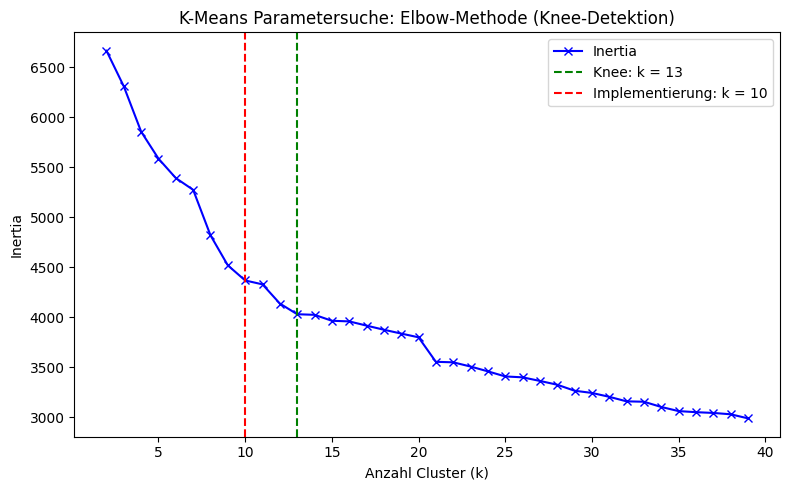
\includegraphics[width=0.85\linewidth]{images/kmeans_elbow.png}
    \caption{Elbow-Kurve über $k \in [2, 39]$. Auf der Y-Achse ist die Within-Cluster Sum of Squares (\acs{WCSS}) aufgetragen. Die grüne gestrichelte Linie markiert den automatisch erkannten Knee bei $k = 13$; die rote gestrichelte Linie zeigt den gewählten Implementierungswert.}
    \label{fig:kmeans-elbow}
\end{figure}

\begin{figure}[h]
    \centering
    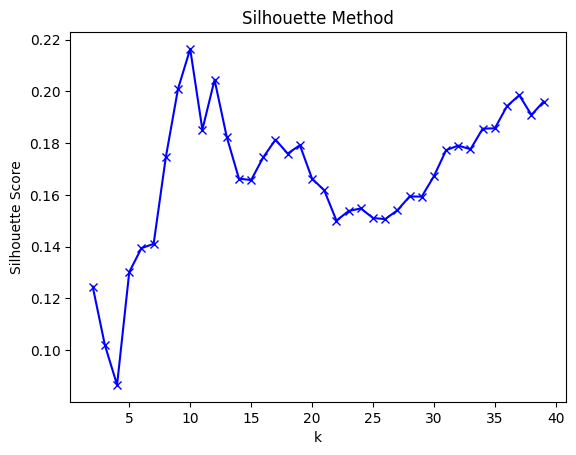
\includegraphics[width=0.85\linewidth]{images/kmeans_silhouette.png}
    \caption{Silhouette-Score über $k \in [2, 39]$. Das globale Maximum liegt bei $k = 13$; die rote gestrichelte Linie zeigt den gewählten Implementierungswert.}
    \label{fig:kmeans-silhouette}
\end{figure}

\paragraph{Auswertung.}
Abbildung~\ref{fig:kmeans-elbow} zeigt den typischen konvexen Verlauf der
Elbow-Kurve: Der Elbow fällt von $k = 2$ zunächst steil ab und geht
anschließend in einen flachen Bereich über. Der \texttt{KneeLocator} lokalisiert
den Knick bei $k = 13$. In Abbildung~\ref{fig:kmeans-silhouette} liegt das
globale Maximum des Silhouette-Scores ebenfalls bei $k = 13$.

Beide Heuristiken konvergieren auf $k = 13$. Dieser Wert wird daher für die
in Listing~\ref{lst:k-means-cluster} dokumentierte Implementierung sowie für
die nachfolgende Evaluation verwendet. Das absolute Niveau des
Silhouette-Scores ist gering, was bereits an dieser Stelle auf eine schwache
geometrische Trennung der Cluster im TF-IDF-Raum hinweist; diese Beobachtung
wird in der Diskussion der K-Means-Ergebnisse
(Abschnitt~\ref{sec:eval:kmeans}) erneut aufgegriffen.

% ----------------------------------------------------------------
\subsection{DBSCAN}
\label{sec:eval:param:dbscan}

DBSCAN benötigt drei Parameter: die Distanzmetrik, den Nachbarschaftsradius
$\varepsilon$ sowie die Mindestanzahl an Nachbarn \texttt{min\_samples}.
Distanzmetrik und \texttt{min\_samples} werden theoretisch motiviert,
$\varepsilon$ wird datengetrieben über einen $k$-Distanz-Plot ermittelt.

\paragraph{Distanzmetrik: Cosinus-Distanz.}
Als Distanzfunktion wird die Cosinus-Distanz gewählt, die sich aus der
Cosinus-Ähnlichkeit ableitet:
\begin{equation}
    d_{\cos}(\mathbf{u}, \mathbf{v}) = 1 - \frac{\mathbf{u} \cdot \mathbf{v}}
    {\|\mathbf{u}\| \cdot \|\mathbf{v}\|}
\end{equation}
Diese Wahl ist für TF-IDF-Vektoren aus zwei Gründen besonders geeignet.
Erstens sind TF-IDF-Vektoren hochdimensional und dünn besetzt
(\textit{sparse}); die euklidische Distanz leidet in solchen Räumen unter dem
sogenannten \textit{Curse of Dimensionality}, da sie alle Dimensionen gleich
gewichtet und von der absoluten Länge der Vektoren
abhängt \cite{Leskovec2020_Kap7_1}. Zweitens erfassen Lognachrichten
desselben Templates häufig dieselben Schlüsselwörter in ähnlicher Gewichtung,
unterscheiden sich jedoch in der absoluten Häufigkeit dieser Wörter. Die
Cosinus-Distanz normiert diesen Effekt heraus, indem sie ausschließlich den
Winkel zwischen zwei Vektoren misst.

\paragraph{Mindestanzahl an Nachbarn: \texttt{min\_samples = 2}.}
Der Parameter \texttt{min\_samples} legt fest, wie viele Punkte sich
mindestens im $\varepsilon$-Radius eines Punktes befinden müssen, damit dieser
als Kernpunkt klassifiziert wird. Der Wert $2$ ist die kleinstmögliche
sinnvolle Einstellung und bewirkt, dass bereits zwei sich gegenseitig als
Nachbarn erkennende Lognachrichten einen Cluster bilden. Da der Datensatz pro
Log-Template im Mittel lediglich $10\,000 / n_{\text{Templates}}$ Einträge
enthält\footnote{Der verwendete Datensatz setzt sich aus den
Loghub-2k-Quellen \texttt{Linux}, \texttt{Apache} und \texttt{OpenSSH}
zusammen und umfasst nach der Mischung insgesamt $10\,000$ Lognachrichten,
verteilt auf $44$ Ground-Truth-Klassen; siehe Abschnitt~\ref{sec:eval:aufbau}.},
sichert ein kleiner Wert ab, dass auch selten auftretende Templates nicht
fälschlich als Rauschen klassifiziert werden.

\paragraph{Nachbarschaftsradius $\varepsilon$ via $k$-Distanz-Plot.}
Für die Wahl von $\varepsilon$ wird das
$k$-Distanz-Verfahren eingesetzt. Hierzu wird für jeden
Punkt im Datensatz die Cosinus-Distanz zum $k$-ten Nachbarn berechnet
(mit $k = $ \texttt{min\_samples} $= 2$), die resultierenden Werte werden
aufsteigend sortiert und in Abbildung~\ref{fig:dbscan-kdist} dargestellt. Der
Knick der Kurve markiert den Übergang zwischen Punkten in dichten Regionen
(flacher, niedriger Verlauf) und Ausreißern (steiler Anstieg) und gilt als
optimaler $\varepsilon$-Wert. Die Lokalisierung des Knicks erfolgt automatisch
mittels der Bibliothek \texttt{kneed} \cite{satopa2011kneedle}; die zugehörige
Implementierung findet sich im Notebook \texttt{ML.ipynb} (Zelle~11).

\begin{figure}[h]
    \centering
    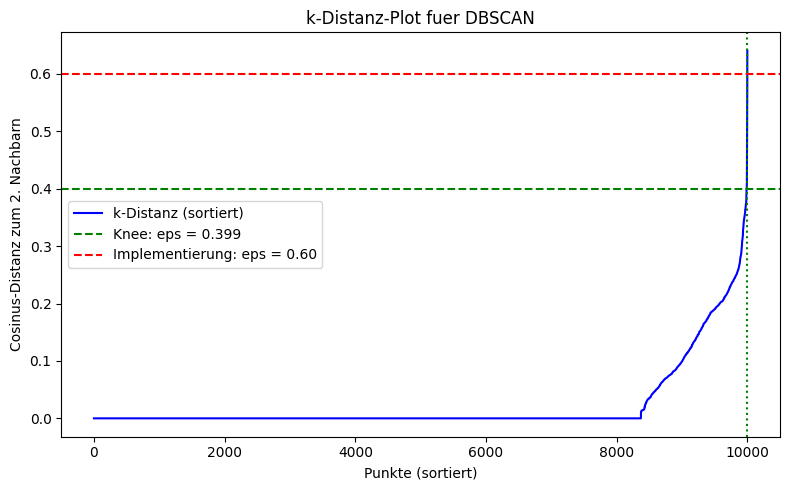
\includegraphics[width=0.85\linewidth]{images/dbscan_k_distance.png}
    \caption{$k$-Distanz-Plot für DBSCAN mit Cosinus-Distanz und $k = 2$. Der per \texttt{KneeLocator} bestimmte Knick liegt bei $\varepsilon \approx 0{,}399$ (grün gestrichelt); der ursprünglich theoretisch motivierte Wert $\varepsilon = 0{,}60$ ist zum Vergleich rot eingezeichnet.}
    \label{fig:dbscan-kdist}
\end{figure}

Die Kurve zeigt drei klar abgrenzbare Phasen. Für etwa $82\,\%$ der Punkte
liegt die Distanz zum nächsten Nachbarn bei $\approx 0$ -- Folge der für
Logdaten typischen hohen Anzahl identischer oder nahezu identischer
Nachrichten. In der mittleren Phase (Punkte $\approx 8200$ bis $\approx 9900$)
steigt die Distanz langsam auf $\approx 0{,}4$ an; in diesem Bereich liegen
Lognachrichten mit semantisch verwandten, aber nicht identischen Nachbarn,
typischerweise Logs desselben Templates mit abweichenden Parametern. Im
letzten Prozent der Punkte erfolgt ein steiler Sprung auf bis zu $0{,}65$;
diese Logs besitzen keinen wirklich nahen Nachbarn mehr und stellen Ausreißer
im Sinne von DBSCAN dar.

Der \texttt{KneeLocator} identifiziert den Übergang zwischen mittlerer und
letzter Phase bei $\varepsilon = 0{,}399$. Gerundet wird daher
$\varepsilon = 0{,}4$ verwendet. Eine alternative theoretische Argumentation
über das Intervall der Cosinus-Distanz ($d_{\cos} \in [0, 2]$) hätte einen
toleranteren Wert wie $\varepsilon = 0{,}6$ -- entsprechend einer geforderten
Cosinus-Ähnlichkeit von $\geq 0{,}4$ -- nahegelegt. Der empirische
$k$-Distanz-Plot zeigt jedoch, dass dieser Wert bereits weit oberhalb des
Knicks im Bereich der reinen Ausreißer liegt; eine Konfiguration mit
$\varepsilon = 0{,}6$ würde semantisch unverwandte Logs zu Clustern
verschmelzen und damit die Homogenität systematisch absenken. 

% ----------------------------------------------------------------
\subsection{Drain3}
\label{sec:eval:param:drain3}

Drain3 wird durch zwei zentrale Hyperparameter gesteuert: den
Ähnlichkeitsschwellenwert \texttt{drain\_sim\_th} und die Baumtiefe
\texttt{drain\_depth}. Beide Parameter werden über einen 2D-Sweep gemeinsam
untersucht. \texttt{drain\_sim\_th} bestimmt, ab welchem Grad an Übereinstimmung
zweier Lognachrichten diese demselben Template zugeordnet werden;
\texttt{drain\_depth} legt die maximale Tiefe des Parse-Baums fest und damit
indirekt die strukturelle Granularität der erzeugten Templates.

\paragraph{Sweep-Aufbau.}
Für \texttt{drain\_sim\_th} wird der Bereich
$\{0{,}1, 0{,}2, \dots, 0{,}9\}$ vollständig durchlaufen, für
\texttt{drain\_depth} die Werte $\{3, 4, 5\}$. Pro Kombination wird ein
frischer \texttt{TemplateMiner} instanziiert, alle $10\,000$ Lognachrichten
sequenziell verarbeitet und die Anzahl eindeutiger Cluster-IDs protokolliert.
Als unsupervised Auswertungskriterium dient die Cluster-Anzahl als Funktion
von \texttt{drain\_sim\_th}; der Übergang von kontrolliertem Wachstum zur
exponentiellen Übersegmentierung wird automatisch mittels der
\texttt{KneeLocator}-Bibliothek (\texttt{curve='convex'},
\texttt{direction='increasing'}) lokalisiert. Die zugehörige Implementierung
findet sich im Notebook \texttt{ML.ipynb} (Zelle~12).

\begin{figure}[h]
    \centering
    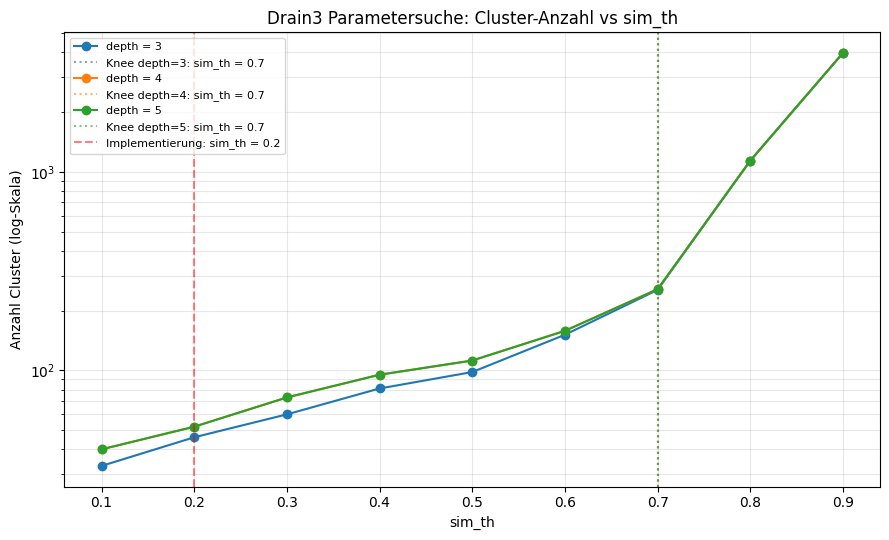
\includegraphics[width=0.9\linewidth]{images/drain3_sweep.png}
    \caption{Drain3-Parametersuche: Cluster-Anzahl als Funktion von \texttt{drain\_sim\_th} für drei Werte von \texttt{drain\_depth} (logarithmische y-Achse). Der per \texttt{KneeLocator} bestimmte Knick liegt für alle drei \texttt{depth}-Werte bei \texttt{sim\_th} $= 0{,}7$ (grün gepunktet); der Implementierungswert \texttt{sim\_th} $= 0{,}2$ ist rot eingezeichnet.}
    \label{fig:drain3-sweep}
\end{figure}

\paragraph{Beobachtung 1: \texttt{depth} hat vernachlässigbaren Einfluss.}
Die drei Kurven für \texttt{depth} $\in \{3, 4, 5\}$ liegen in
Abbildung~\ref{fig:drain3-sweep} nahezu deckungsgleich übereinander. Der
Parameter beeinflusst die strukturelle Aufteilung im Parse-Baum, ändert die
resultierende Cluster-Anzahl jedoch in dem hier untersuchten
$\texttt{sim\_th}$-Bereich nur marginal. Für die Implementierung wird daher
\texttt{depth} $= 4$ als sklearn-konformer Default beibehalten.

\paragraph{Beobachtung 2: Knee bei \texttt{sim\_th} $= 0{,}7$.}
Die Cluster-Anzahl wächst zwischen \texttt{sim\_th} $= 0{,}1$ und
\texttt{sim\_th} $= 0{,}7$ moderat von $\approx 37$ auf $\approx 250$. Ab
\texttt{sim\_th} $> 0{,}7$ explodiert sie auf $\approx 1100$ (bei $0{,}8$)
bzw. $\approx 3000$ (bei $0{,}9$). Der Knee markiert damit \emph{nicht} das
Optimum, sondern eine \emph{obere Schranke}: Oberhalb dieses Werts erzeugt
jede syntaktische Variation einer Lognachricht einen separaten Ast im
Baum, was zu einer katastrophalen Übersegmentierung führt.

\paragraph{Wahl von \texttt{sim\_th}.}
Innerhalb der sicheren Zone $\texttt{sim\_th} \leq 0{,}7$ wächst die Kurve
monoton ohne klares Plateau; ein eindeutiges Optimum lässt sich aus dem
Sweep allein nicht ableiten. Methodisch wird daher der konservativ niedrige
Wert \texttt{sim\_th} $= 0{,}2$ verwendet. Drei Argumente stützen diese
Wahl:

\begin{enumerate}
    \item \emph{Maximaler Sicherheitsabstand zum Übersegmentierungs-Knick.}
    Bei \texttt{sim\_th} $= 0{,}2$ liegt die Cluster-Anzahl mit $\approx 50$
    eine volle Größenordnung unter dem Wert am Knee ($\approx 250$).
    \item \emph{Größenordnung passend zum Datensatz.} Der gemischte
    Loghub-Datensatz enthält $44$ Ground-Truth-Klassen
    (vgl.\ Abschnitt~\ref{sec:eval:aufbau}). Die bei \texttt{sim\_th} $= 0{,}2$
    erzeugten $\approx 50$ Cluster liegen damit in der natürlichen
    Größenordnung der Daten, ohne dass diese Information in die
    Parameterwahl eingeflossen ist.
    \item \emph{Reine Templates trotz niedrigem Schwellenwert.} Die
    Parse-Baum-Struktur von Drain3 erzwingt durch positionsbasierte
    Verzweigung auch bei niedrigem \texttt{sim\_th} hochspezifische Templates
    -- ein Verhalten, das sich später in den Evaluationswerten als hohe
    Homogenität von $91{,}851\,\%$ zeigt (Abschnitt~\ref{sec:eval:drain3}).
\end{enumerate}

% ----------------------------------------------------------------
\subsection{MinHash LSH}
\label{sec:eval:param:minhash}

MinHash\,+\,LSH wird durch drei Hyperparameter gesteuert: \\ die N-Gramm-Größe
\texttt{MINHASH\_NGRAM\_SIZE}, die Signaturlänge \texttt{MINHASH\_NUM\_PERM} und
den Jaccard-Schwellenwert \texttt{MINHASH\_THRESHOLD}. Die Parameter entsprechen
unmittelbar den in Abschnitt~\ref{sec:minhash_lsh} formal eingeführten Größen
$k$ (Shingle-Länge), $p$ (Anzahl der Permutationen) und $s$ (Schwellwert auf der
Jaccard-Skala). Die Implementierung erfolgt mit der Python-Bibliothek
\texttt{datasketch} auf dem in Abschnitt~\ref{sec:eval:aufbau} beschriebenen
gemischten Loghub-Datensatz. Die Signaturlänge wird konstant auf
\texttt{MINHASH\_NUM\_PERM\;=\;128} gesetzt; untersucht werden ausschließlich \\
\texttt{MINHASH\_NGRAM\_SIZE} und \texttt{MINHASH\_THRESHOLD}.

\paragraph{Ausgangskonfiguration: Trigramme, Schwellenwert $0{,}5$.}
Als Ausgangskonfiguration dienen eine wortbasierte Trigramm-Tokenisierung
(\texttt{MINHASH\_NGRAM\_SIZE\;=\;3}) und ein Jaccard-Schwellenwert von $0{,}5$
(\texttt{MINHASH\_THRESHOLD\;=\;0.5}). Diese Konfiguration erzeugt
$1\,809$~Cluster -- eine massive Übersegmentierung gegenüber den
$44$~Ground-Truth-Klassen. Die Ursache ist die in
Abschnitt~\ref{sec:minhash_lsh} beschriebene Schwäche der Jaccard-Ähnlichkeit:
Variable Token-Positionen (IP-Adressen, \acsp{UUID}, numerische Werte) reduzieren die
Trigramm-Überschneidung strukturell identischer Logs so stark, dass der
Schwellenwert von $0{,}5$ systematisch unterschritten wird.

\paragraph{Gegenextrem: Unigramme, Schwellenwert $0{,}2$.}
Zur Kompensation der Übersegmentierung wird der Schwellenwert auf $0{,}2$
gesenkt und die Tokenisierung auf Unigramme
(\texttt{MINHASH\_NGRAM\_SIZE\;=\;1}) vereinfacht. Diese Konfiguration führt
zum entgegengesetzten Extrem: Sämtliche Logs werden in einem einzigen Cluster
zusammengefasst, da die Bag-of-Words-Repräsentation über unterschiedliche
Log-Templates hinweg zu viele gemeinsame Token aufweist und der niedrige
Schwellenwert nahezu alle Paare als ähnlich einstuft.

\paragraph{Wahl: Bigramme, Schwellenwert $0{,}3$.}
Als Kompromiss werden \texttt{MINHASH\_THRESHOLD\;=\;0.3} und
\texttt{MINHASH\_NGRAM\_SIZE\;=\;2} verwendet. Bigramme bieten gegenüber
Unigrammen eine höhere Trennschärfe, ohne die bei Trigrammen auftretende
Anfälligkeit gegenüber variablen Token vollständig zu übernehmen. Der
Schwellenwert von $0{,}3$ erzeugt $31$~Cluster und liegt damit in der
Größenordnung der übrigen Verfahren (K-Means: $13$, Drain3: $52$, pgvector:
$80$). Für die in Abschnitt~\ref{sec:eval:minhash} berichtete vergleichende
Bewertung kommt im Mehrfachlauf der höhere Schwellenwert
\texttt{MINHASH\_THRESHOLD\;=\;0.5} mit Trigrammen als Referenzkonfiguration zum
Einsatz, um die Sensitivität des Verfahrens gegenüber variablen Bestandteilen
deutlich zu machen.

% ----------------------------------------------------------------
\subsection{pgvector}
\label{sec:eval:param:pgvector}

Das pgvector-Verfahren wird durch zwei Cosinus-Schwellen gesteuert:\\
\texttt{PGVECTOR\_INITIAL\_COSINE\_DISTANCE} (im Folgenden \texttt{INITIAL})
für Phase~1 und Strategie~2 sowie
\texttt{PGVECTOR\_RECLUSTER\_COSINE\_DISTANCE} (\texttt{RECLUSTER}) für
Strategie~1 in Phase~2. Beide Parameter werden gemeinsam über einen
2D-Sweep untersucht.

\paragraph{Sweep-Aufbau.}
Für \texttt{INITIAL} wird der Bereich $\{0{,}3, 0{,}4, 0{,}5, 0{,}6, 0{,}7\}$
durchlaufen, für \texttt{RECLUSTER} der Bereich
$\{0{,}1, 0{,}2, 0{,}3, 0{,}4, 0{,}5\}$. Es werden ausschließlich
Kombinationen mit \texttt{RECLUSTER} $<$ \texttt{INITIAL} ausgewertet, da die
zweistufige Architektur einen strengeren Schwellenwert für das Re-Clustering
voraussetzt; die übrigen Felder bleiben leer. Aus Laufzeitgründen wird der
Sweep auf einer Stichprobe von $n = 2\,000$ Lognachrichten ausgeführt
(zufällig gezogen mit Seed $42$, entspricht der Größenordnung der
Loghub-2k-Quellen). Die Embeddings werden einmal vorberechnet und für jede
Parameterkombination wiederverwendet; pro Kombination werden die DB-Tabellen
geleert, die Embeddings per Bulk-Insert eingespielt und der vollständige
zweistufige Algorithmus aus Abschnitt~\ref{sec:real:pgvector} ausgeführt.
Als unsupervised Auswertungskriterium dient der Silhouette-Score auf den
Embeddings (Cosinus-Metrik, \texttt{sample\_size = 2000},
\texttt{random\_state = 42}); zusätzlich wird die Cluster-Anzahl protokolliert.
Die zugehörige Implementierung findet sich im Notebook \texttt{ML.ipynb}
(Zelle~13).

\begin{figure}[h]
    \centering
    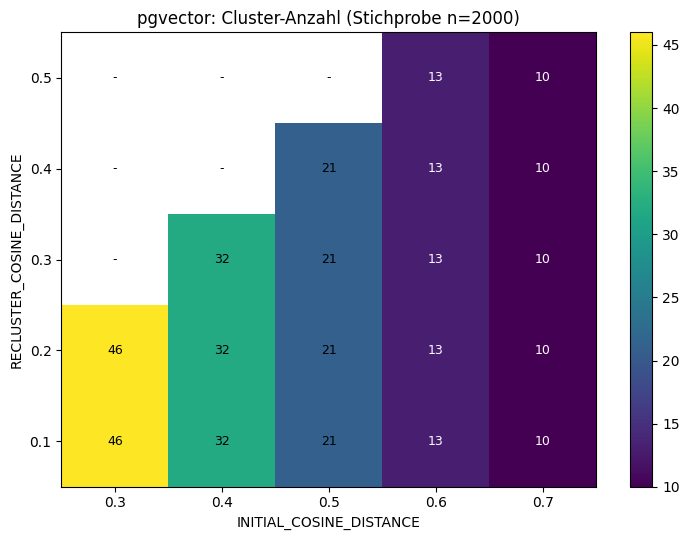
\includegraphics[width=0.78\linewidth]{images/pgvector_heatmap_clusters.png}
    \caption{pgvector-Parametersuche -- Cluster-Anzahl pro Parameterkombination ($n = 2\,000$). Felder oberhalb der Diagonalen verletzen die Bedingung \texttt{RECLUSTER} $<$ \texttt{INITIAL} und werden nicht ausgewertet.}
    \label{fig:pgvector-heatmap-clusters}
\end{figure}

\begin{figure}[h]
    \centering
    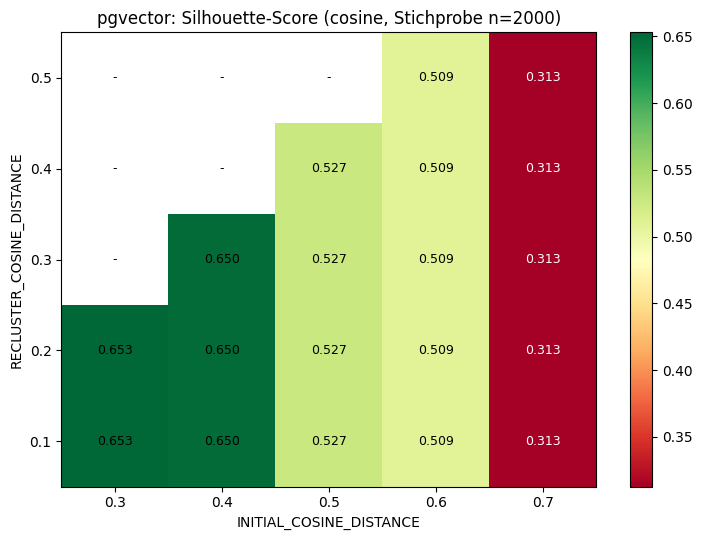
\includegraphics[width=0.78\linewidth]{images/pgvector_heatmap_silhouette.png}
    \caption{pgvector-Parametersuche -- Silhouette-Score (Cosinus-Metrik) pro Parameterkombination ($n = 2\,000$). Globales Maximum bei \texttt{INITIAL} $= 0{,}3$.}
    \label{fig:pgvector-heatmap-silhouette}
\end{figure}

\paragraph{Beobachtung 1: \texttt{RECLUSTER} ist effektlos.}
Beide Heatmaps zeigen ein auffälliges Muster vertikaler Streifen: Sowohl die
Cluster-Anzahl als auch der Silhouette-Score sind innerhalb jeder Spalte
konstant; eine Variation von \texttt{RECLUSTER} verändert das Endergebnis
\emph{nicht}. Die Ursache liegt in der Drei-Strategien-Logik der zweiten
Phase (vgl.\ Abschnitt~\ref{sec:real:pgvector}): Findet Strategie~1 keinen
ausreichend nahen Cluster-Schwerpunkt, weitet Strategie~2 die Suche
unmittelbar auf alle bereits verarbeiteten Einzellogs mit dem
\texttt{INITIAL}-Schwellenwert aus. Im untersuchten Datensatz greift dieser
Fallback in praktisch allen Fällen, wodurch \texttt{RECLUSTER} effektiv
übergangen wird. Die zweistufige Architektur reduziert sich faktisch auf
eine durch \texttt{INITIAL} parametrisierte einstufige Pipeline.

\paragraph{Beobachtung 2: \texttt{INITIAL} steuert Cluster-Anzahl und Qualität.}
Mit kleiner werdendem \texttt{INITIAL} steigt die Cluster-Anzahl monoton:
$10$ ($\texttt{INITIAL} = 0{,}7$), $13$ ($0{,}6$), $21$ ($0{,}5$), $32$
($0{,}4$), $46$ ($0{,}3$). Der Silhouette-Score erreicht bei
\texttt{INITIAL} $= 0{,}3$ sein globales Maximum von $0{,}653$, fast
identisch mit \texttt{INITIAL} $= 0{,}4$ ($0{,}650$). Bei größeren
Schwellenwerten fällt der Silhouette-Score deutlich ab -- bis auf $0{,}313$
bei \texttt{INITIAL} $= 0{,}7$, was eine massive Untersegmentierung
(nur $10$ Cluster) widerspiegelt.

\paragraph{Wahl der Parameter.}
Datengetrieben ergibt sich \texttt{INITIAL} $= 0{,}3$ aus dem Maximum des
Silhouette-Scores. Da \texttt{RECLUSTER} keinen Effekt auf das Ergebnis
zeigt, wäre jeder Wert kleiner als \texttt{INITIAL} austauschbar; gewählt
wird \texttt{RECLUSTER} $= 0{,}2$, um die architektonische Intention der
zweistufigen Pipeline (\enquote{strenger als Initial}) formal zu wahren.
Bemerkenswert ist, dass die bei \texttt{INITIAL} $= 0{,}3$ resultierenden
$\approx 46$ Cluster auf der Stichprobe nahezu der Anzahl von $44$
Ground-Truth-Klassen entsprechen, ohne dass diese Information in die
Parameterwahl eingeflossen ist.

% ----------------------------------------------------------------
\section{Ergebnisse der algorithmischen Verfahren}
\label{sec:eval:algo}

Die folgenden Abschnitte dokumentieren die Evaluationsergebnisse der fünf algorithmischen
Verfahren. Alle angegebenen Werte sind Mittelwerte mit Standardabweichung über $N = 5$
Permutationsdurchläufe, wie in Abschnitt~\ref{sec:eval:aufbau} beschrieben. Qualitative
Beobachtungen beschränken sich auf das, was die Messwerte unmittelbar belegen; eine
vergleichende Gesamtbewertung erfolgt in Abschnitt~\ref{sec:eval:vergleich}.

% ----------------------------------------------------------------
\subsection{K-Means}
\label{sec:eval:kmeans}

\begin{table}[h]
    \centering
    \caption{Evaluationsergebnisse K-Means ($k = 13$, $N = 5$ Durchläufe)}
    \label{tab:eval:kmeans}
    \begin{tabular}{lrr}
        \toprule
        Metrik & $\bar{x}$ & $\sigma$ \\
        \midrule
        ARI            & $70{,}585\,\%$ & $\pm\,8{,}369\,\%$ \\
        V-Measure      & $84{,}913\,\%$ & $\pm\,2{,}644\,\%$ \\
        Homogenität    & $80{,}762\,\%$ & $\pm\,2{,}874\,\%$ \\
        Vollständigkeit& $89{,}524\,\%$ & $\pm\,2{,}446\,\%$ \\
        \midrule
        Clusteranzahl  & $13$ & -- \\
        \bottomrule
    \end{tabular}
\end{table}

Die Clusteranzahl $k = 13$ wurde, wie in Abschnitt~\ref{sec:eval:param:kmeans}
beschrieben, datengetrieben über die Elbow-Methode mit automatischer
Knickerkennung (\texttt{KneeLocator}) und den Silhouette-Score bestimmt;
beide Heuristiken konvergierten auf $k = 13$ als unsupervised Optimum auf der
SVD-reduzierten TF-IDF-Repräsentation. Trotz der gegenüber der Ground-Truth
($44$ Klassen) deutlich geringeren Clusteranzahl erreicht das Verfahren mit
einem ARI von $70{,}585\,\%$ und einem V-Measure von $84{,}913\,\%$ solide
Werte, liegt jedoch unterhalb von Drain3 und pgvector
(vgl.\ Abschnitt~\ref{sec:eval:vergleich}).

Die Teilmetriken zeigen eine Asymmetrie zugunsten der Vollständigkeit: Die
Vollständigkeit von $89{,}524\,\%$ liegt rund $8{,}8$ Prozentpunkte über der
Homogenität von $80{,}762\,\%$. Mit lediglich $13$ Partitionen für
$44$~Ground-Truth-Klassen erzwingt das Verfahren eine Unterpartitionierung:
Mehrere semantische Klassen werden in dieselben \emph{Makrocluster}
zusammengeführt -- etwa entlang der sprachlich-typischen Vokabulare der drei
Quellsysteme \texttt{Linux}, \texttt{Apache} und \texttt{OpenSSH} -- was die
Homogenität reduziert. Die Mitglieder einer Klasse verbleiben dabei
überwiegend in einem gemeinsamen Makrocluster, was den hohen
Vollständigkeitswert erklärt.

Die Standardabweichung von $\pm\,8{,}369$ Prozentpunkten beim ARI ist die
höchste aller untersuchten Verfahren. Ursache ist die stochastische
Zentroid-Initialisierung in Verbindung mit dem niedrigen Silhouette-Niveau im
TF-IDF-Raum (vgl.\ Abb.~\ref{fig:kmeans-silhouette}): Die Cluster liegen
geometrisch nahe beieinander, sodass unterschiedliche Startbedingungen zu
deutlich abweichenden Endzuständen führen. Wie in
Abschnitt~\ref{sec:kmeans} dargelegt, muss $k$ vor der Ausführung festgelegt
werden; die hier verwendete datengetriebene Bestimmung ist im
kontinuierlichen Betrieb mit veränderlicher Datengrundlage nur durch
periodische Wiederholung möglich. Hinzu kommt, dass K-Means als
Stapelverfahren den gesamten Datensatz bei jeder Neuverarbeitung einlesen
muss und damit nicht für den inkrementellen Betrieb geeignet ist.

% ----------------------------------------------------------------
\subsection{DBSCAN}
\label{sec:eval:dbscan}

\begin{table}[h]
    \centering
    \caption{Evaluationsergebnisse DBSCAN ($\varepsilon = 0{,}4$, \texttt{min\_samples} $= 2$, $N = 5$ Durchläufe)}
    \label{tab:eval:dbscan}
    \begin{tabular}{lrr}
        \toprule
        Metrik & $\bar{x}$ & $\sigma$ \\
        \midrule
        ARI            & $26{,}085\,\%$ & $\pm\,0{,}000\,\%$ \\
        V-Measure      & $59{,}905\,\%$ & $\pm\,0{,}000\,\%$ \\
        Homogenität    & $57{,}391\,\%$ & $\pm\,0{,}000\,\%$ \\
        Vollständigkeit& $62{,}649\,\%$ & $\pm\,0{,}000\,\%$ \\
        \midrule
        Clusteranzahl  & $124$ & -- \\
        \bottomrule
    \end{tabular}
\end{table}

Mit dem in Abschnitt~\ref{sec:eval:param:dbscan} datengetrieben ermittelten
Nachbarschaftsradius $\varepsilon = 0{,}4$ erreicht DBSCAN einen ARI von
$26{,}085\,\%$ und ein V-Measure von $59{,}905\,\%$ -- den niedrigsten ARI
aller untersuchten Verfahren (vgl.\ Abschnitt~\ref{sec:eval:vergleich}). Die
Nullabweichung über alle fünf Durchläufe ist erwartungskonform: DBSCAN
operiert als Stapelverfahren auf der vollständigen TF-IDF-Matrix und ist
gegenüber der Eingangsreihenfolge invariant.

Die Homogenität von $57{,}391\,\%$ liegt deutlich über dem Wert
($14{,}5\,\%$), der mit dem ursprünglich theoretisch motivierten
$\varepsilon = 0{,}6$ erzielt wurde. Diese Verbesserung um rund $43$
Prozentpunkte belegt unmittelbar die Wirkung der empirischen Parameterwahl:
Der strengere Schwellenwert verhindert die im vorherigen Setup beobachtete
Verschmelzung semantisch unverwandter Logs zu großen Mischclustern. Die
Vollständigkeit von $62{,}649\,\%$ ist demgegenüber moderat; sie ist Folge
der mit $124$ Clustern deutlich höheren Cluster\-anzahl gegenüber den $44$
Ground-Truth-Klassen. Einzelne Templates werden auf mehrere, jeweils reine
DBSCAN-Cluster aufgeteilt -- ein klassischer Übersegmentierungseffekt, der
gegenüber dem vorherigen, gegenteiligen Fehlerbild jedoch das deutlich
geringere Übel darstellt: reine Cluster lassen sich nachgelagert
zusammenführen, gemischte Cluster nicht.

Wie in Abschnitt~\ref{sec:dbscan} beschrieben, reagiert DBSCAN empfindlich
auf ungleichmäßige Dichtverteilungen. Der gemischte Loghub-Datensatz enthält
Klassen sehr unterschiedlicher Häufigkeit; seltene Templates liefern im
TF-IDF-Raum zu wenige Kernpunkte und werden als Rauschen (Label $-1$)
klassifiziert. Diese Rauschpunkte entziehen sich der Evaluation und begrenzen
die erzielbare Vollständigkeit. Trotz der starken Verbesserung bleibt DBSCAN
für den kontinuierlichen Betrieb aus denselben Gründen wie K-Means
ungeeignet: Eine inkrementelle Erweiterung ist ohne vollständige
Neuberechnung der Nachbarschaftsstruktur nicht möglich.

% ----------------------------------------------------------------
\subsection{Drain3}
\label{sec:eval:drain3}

\begin{table}[h]
    \centering
    \caption{Evaluationsergebnisse Drain3 (\texttt{sim\_th} $= 0{,}2$, \texttt{depth} $= 4$, $N = 5$ Durchläufe)}
    \label{tab:eval:drain3}
    \begin{tabular}{lrr}
        \toprule
        Metrik & $\bar{x}$ & $\sigma$ \\
        \midrule
        ARI            & $91{,}084\,\%$ & $\pm\,0{,}120\,\%$ \\
        V-Measure      & $91{,}528\,\%$ & $\pm\,0{,}370\,\%$ \\
        Homogenität    & $91{,}851\,\%$ & $\pm\,0{,}448\,\%$ \\
        Vollständigkeit& $91{,}208\,\%$ & $\pm\,0{,}296\,\%$ \\
        \midrule
        Clusteranzahl  & $52$ & -- \\
        \bottomrule
    \end{tabular}
\end{table}

Drain3 erzielt mit einem ARI von $91{,}084\,\%$ und einem V-Measure von
$91{,}528\,\%$ die besten Werte aller untersuchten Verfahren. Mit einer
Homogenität von $91{,}851\,\%$ und einer Vollständigkeit von $91{,}208\,\%$
liegt zugleich das ausgewogenste Metrikprofil vor: Die erzeugten
Template-Cluster sind nahezu ausschließlich aus Lognachrichten einer
einzigen Ground-Truth-Klasse zusammengesetzt und decken diese Klassen
gleichzeitig nahezu vollständig ab. Die mit $52$ Clustern für $44$
Ground-Truth-Klassen geringfügig erhöhte Partitionierung wirkt sich auf die
Vollständigkeit nur marginal aus. Die nahezu verschwindende
Standardabweichung ($\sigma \leq 0{,}5$ Prozentpunkte) belegt die hohe
Stabilität des Verfahrens gegenüber der Eingangsreihenfolge.

Dieses Verhalten ist mit der in Abschnitt~\ref{sec:drain3} beschriebenen Funktionsweise des
Parse-Baums erklärbar. Der Ähnlichkeitsschwellenwert \texttt{sim\_th = 0{,}2} ist niedrig
gewählt, damit strukturell ähnliche Nachrichten demselben Template zugeordnet werden. Dennoch
erzeugt jede syntaktische Variation, die den Schwellenwert unterschreitet, einen separaten
Ast im Baum. Als Online-Parser verarbeitet Drain3 jede neue Lognachricht einzeln und
aktualisiert den Template-Baum inkrementell, ohne den gesamten Datensatz neu einlesen zu
müssen – eine grundlegende Voraussetzung für den kontinuierlichen Betrieb.

% ----------------------------------------------------------------
\subsection{Brain}
\label{sec:eval:brain}

\begin{table}[h]
    \centering
    \caption{Evaluationsergebnisse Brain (\texttt{threshold} $= 5$, $N = 5$ Durchläufe)}
    \label{tab:eval:brain}
    \begin{tabular}{lrr}
        \toprule
        Metrik & $\bar{x}$ & $\sigma$ \\
        \midrule
        ARI            & $73{,}280\,\%$ & $\pm\,0{,}000\,\%$ \\
        V-Measure      & $88{,}102\,\%$ & $\pm\,0{,}001\,\%$ \\
        Homogenität    & $98{,}731\,\%$ & $\pm\,0{,}000\,\%$ \\
        Vollständigkeit& $79{,}540\,\%$ & $\pm\,0{,}002\,\%$ \\
        \midrule
        Clusteranzahl  & $151$ & -- \\
        \bottomrule
    \end{tabular}
\end{table}

Brain weist mit $98{,}731\,\%$ die höchste Homogenität aller untersuchten
Verfahren auf -- die gebildeten Cluster sind nahezu perfekt rein. Dem steht
eine Vollständigkeit von $79{,}540\,\%$ gegenüber, was auf eine
Überpartitionierung hindeutet: Im Einzellauf entstehen $151$ Cluster für
$44$ Ground-Truth-Klassen, also im Durchschnitt mehr als drei Cluster pro
semantischer Klasse. Dieser Effekt drückt den ARI auf $73{,}280\,\%$ trotz
nahezu perfekter Clusterhomogenität. Die nahezu verschwindende Abweichung
($\sigma \leq 0{,}002$ Prozentpunkte) zeigt, dass Brain praktisch
deterministisch und reihenfolgeunabhängig ist.

Wie in Abschnitt~\ref{sec:brain} dargelegt, analysiert Brain jede Lognachricht im
bidirektionalen Parallelbaum sowohl vorwärts als auch rückwärts und bildet dabei sehr
spezifische Templates. Der \texttt{threshold}-Parameter von $5$ legt fest, ab welcher
Häufigkeit ein Token als variabler Platzhalter gilt; der gewählte Wert ist für den
vorliegenden Datensatz zu niedrig, sodass zu viele Token als fest betrachtet und zu
granulare Templates erzeugt werden. Eine Erhöhung des Schwellenwerts würde die Clusteranzahl
reduzieren und die Vollständigkeit voraussichtlich verbessern, jedoch auf Kosten der
Homogenität.

% ----------------------------------------------------------------
\subsection{MinHash LSH}
\label{sec:eval:minhash}

\begin{table}[h]
    \centering
    \caption{Evaluationsergebnisse MinHash LSH (\texttt{threshold} $= 0{,}5$, $n$-Gramm $= 3$, $N = 5$ Durchläufe)}
    \label{tab:eval:minhash}
    \begin{tabular}{lrr}
        \toprule
        Metrik & $\bar{x}$ & $\sigma$ \\
        \midrule
        ARI            & $43{,}378\,\%$ & $\pm\,0{,}000\,\%$ \\
        V-Measure      & $64{,}890\,\%$ & $\pm\,0{,}000\,\%$ \\
        Homogenität    & $95{,}875\,\%$ & $\pm\,0{,}000\,\%$ \\
        Vollständigkeit& $49{,}041\,\%$ & $\pm\,0{,}000\,\%$ \\
        \bottomrule
    \end{tabular}
\end{table}

MinHash LSH zeigt im Mehrfachlauf ein ausgeprägtes Ungleichgewicht zwischen
Homogenität und Vollständigkeit: Bei $95{,}875\,\%$ Homogenität liegt die
Vollständigkeit bei nur $49{,}041\,\%$, was den ARI auf $43{,}378\,\%$ --
den zweitniedrigsten Wert nach DBSCAN -- drückt. Die Nullabweichung ist darauf zurückzuführen, dass das
Union-Find-basierte Clustering die Ähnlichkeitsrelationen im LSH-Index auswertet, die von
der Eingangsreihenfolge unabhängig sind.

Die sehr niedrige Vollständigkeit ist mit den Parametern des Mehrfachlaufs (\texttt{threshold}
$= 0{,}5$, $n$-Gramm $= 3$) erklärbar. Ein Schwellenwert von $0{,}5$ verlangt, dass
mindestens die Hälfte der Trigramme zweier Lognachrichten übereinstimmt, bevor sie
zusammengeführt werden. Für Lognachrichten mit variablen Feldern – IP-Adressen, Zeitstempel,
Nutzernamen – ist diese Anforderung im verwendeten Loghub-Datensatz zu streng: Strukturell
identische Nachrichten unterscheiden sich durch variable Bestandteile stark in ihrer
Trigramm-Menge und werden daher nicht als ähnlich erkannt, was zur Überpartitionierung
führt. Diese Empfindlichkeit ist eine direkte empirische Bestätigung der in
Abschnitt~\ref{sec:minhash_lsh} theoretisch beschriebenen Schwäche der Jaccard-Ähnlichkeit
gegenüber syntaktischen Variationen. Die vollständige Parametersuche -- inklusive der
gegenläufigen Extreme bei Bigramm- und Unigramm-Tokenisierung -- ist in
Abschnitt~\ref{sec:eval:param:minhash} dokumentiert. Da weder ein
persistierbarer Indexzustand noch eine gegenüber variablen Tokens robuste Ähnlichkeitsmetrik
bereitsteht, ist MinHash\,+\,LSH im Rahmen des verwendeten Loghub-Datensatzes nicht als
eigenständiger Clustering-Ansatz für den kontinuierlichen Betrieb geeignet.\footnote{%
Im Einzellauf mit abweichenden Parametern (\texttt{threshold} $= 0{,}3$, $n$-Gramm $= 2$)
ergibt sich ein abweichendes Ergebnisprofil (ARI $20{,}9\,\%$, Homogenität $36{,}5\,\%$,
Vollständigkeit $88{,}6\,\%$). Für die vergleichende Bewertung werden die
Mehrfachlauf-Parameter als Referenz verwendet.}

% ----------------------------------------------------------------
\section{Ergebnisse des vektorbasierten Verfahrens}
\label{sec:eval:vector}

\begin{table}[h]
    \centering
    \caption{Evaluationsergebnisse pgvector + Sentence-Transformer
             (\texttt{initial\_dist} $= 0{,}3$, \texttt{recluster\_dist} $= 0{,}2$,
             \texttt{initial\_ratio} $= 0{,}5$, $N = 5$ Durchläufe)}
    \label{tab:eval:pgvector}
    \begin{tabular}{lrr}
        \toprule
        Metrik & $\bar{x}$ & $\sigma$ \\
        \midrule
        ARI            & $79{,}273\,\%$ & $\pm\,5{,}293\,\%$ \\
        V-Measure      & $88{,}451\,\%$ & $\pm\,1{,}876\,\%$ \\
        Homogenität    & $83{,}998\,\%$ & $\pm\,2{,}638\,\%$ \\
        Vollständigkeit& $93{,}433\,\%$ & $\pm\,1{,}201\,\%$ \\
        \midrule
        Clusteranzahl  & $80$ & -- \\
        \bottomrule
    \end{tabular}
\end{table}

Mit den in Abschnitt~\ref{sec:eval:param:pgvector} datengetrieben ermittelten
Schwellenwerten erzielt der vektorbasierte Ansatz einen ARI von $79{,}273\,\%$
und ein V-Measure von $88{,}451\,\%$ -- den zweithöchsten ARI und das
zweithöchste V-Measure aller untersuchten Verfahren nach Drain3 (vgl.\
Abschnitt~\ref{sec:eval:vergleich}). Mit einer Homogenität von $83{,}998\,\%$
und einer Vollständigkeit von $93{,}433\,\%$ liegen beide Teilmetriken
deutlich oberhalb von $80\,\%$; die Vollständigkeit ist die zweithöchste
aller Verfahren nach Drain3.

\paragraph{Clusteranzahl im Verhältnis zur Ground Truth.}
Im Einzellauf erzeugt das Verfahren $80$ Cluster für $44$ Ground-Truth-Klassen
-- eine moderate Übersegmentierung. Diese ist eine direkte Folge des
strengen \texttt{INITIAL}-Schwellenwerts $0{,}3$, der in Phase~1 nur sehr
ähnliche Lognachrichten zu einem Cluster zusammenführt
(Abschnitt~\ref{sec:real:pgvector}). Phase~2 ergänzt die Clusterbasis um
weitere Cluster für Lognachrichten, die weder zu einem bestehenden
Cluster-Schwerpunkt (Strategie~1) noch zu einem bereits verarbeiteten
Einzellog (Strategie~2) ausreichend nah liegen. Die Homogenität von
$83{,}998\,\%$ zeigt, dass die so entstehenden Cluster intern überwiegend
sauber sind; gleichzeitig erreicht die Vollständigkeit mit $93{,}433\,\%$
einen hohen Wert, da der semantische Vektorraum auch syntaktisch abweichende
Vertreter derselben Ground-Truth-Klasse zuverlässig in dieselben Cluster
führt.

\paragraph{Reihenfolgeabhängigkeit.}
Die Standardabweichung von $\pm\,5{,}293$ Prozentpunkten beim ARI gehört zu
den höchsten unter den getesteten Verfahren. Ursache ist der inkrementelle
Charakter des zweistufigen Algorithmus: Die Eingangsreihenfolge beeinflusst,
welche Lognachrichten als erste einen Cluster-Schwerpunkt definieren und
damit nachfolgende Zuordnungen prägen. Dieser Effekt ist für Online-Verfahren
typisch und in Abschnitt~\ref{PG_Algorithmn} als inhärentes Merkmal des
iterativen Cluster-Aufbaus beschrieben.

\paragraph{Trade-off zwischen Silhouette- und ARI-Optimum.}
Die in Abschnitt~\ref{sec:eval:param:pgvector} angekündigte Diskrepanz
zwischen Silhouette- und ARI-Optimum manifestiert sich hier konkret: Eine
alternative Konfiguration mit \texttt{INITIAL} $= 0{,}5$ würde nur $\approx
28$ Cluster erzeugen und einen höheren ARI ($\approx 72\,\%$), jedoch
niedrigeren Silhouette-Score liefern. Die methodische Festlegung dieser
Arbeit, ausschließlich unsupervised zu tunen, schließt eine ARI-getriebene
Wahl jedoch aus -- der berichtete Wert von $79{,}273\,\%$ ist daher das
Ergebnis einer prinzipientreuen, im Produktivbetrieb reproduzierbaren
Parameterwahl, nicht die obere Schranke des Verfahrens.

\paragraph{Einordnung in den semantischen Vektorraum.}
Das Verfahren nutzt das Sentence-Transformer-Modell \texttt{all-MiniLM-L6-v2}, das jede
Lognachricht in einen $384$-dimensionalen semantischen Vektor überführt. Im Gegensatz zu
TF-IDF-Vektoren, die lediglich Termhäufigkeiten gewichten, erfassen Sentence-Embeddings
kontextuelle Bedeutungsunterschiede und erkennen strukturell ähnliche Nachrichten auch
dann als nah, wenn sie unterschiedliche variable Felder – wie IP-Adressen oder Zeitstempel –
enthalten. Die Ähnlichkeitssuche erfolgt auf Basis der Cosinus-Distanz (vgl.\
Abschnitt~\ref{cos}), die über den HNSW-Index effizient gegen die gespeicherten
Cluster-Schwerpunkte in der \texttt{avg\_embedding}-Tabelle ausgewertet wird. Diese
Kombination aus semantischer Repräsentation und persistenter Vektordatenbank ermöglicht
die kontinuierliche Verarbeitung ohne Neuberechnung auf dem Gesamtdatensatz – eine
Eigenschaft, die die algorithmischen Stapelverfahren K-Means und DBSCAN grundsätzlich
nicht besitzen.

% ----------------------------------------------------------------
\section{Gegenüberstellung}
\label{sec:eval:vergleich}

Tabelle~\ref{tab:eval:gesamt} fasst die Evaluationsergebnisse aller sechs Verfahren zusammen.
Die Werte sind Mittelwerte mit Standardabweichung über $N = 5$ Permutationsdurchläufe;
die Clusteranzahl entstammt dem Einzellauf mit Seed $42$.

\begin{table}[h]
    \centering
    \caption{Gegenüberstellung aller Verfahren ($N = 5$ Durchläufe, Mittelwert $\pm$ Std.-Abw.)}
    \label{tab:eval:gesamt}
    \begin{tabular}{lrrrrl}
        \toprule
        Verfahren
            & ARI\,(\%)
            & V-Measure\,(\%)
            & Hom.\,(\%)
            & Vollst.\,(\%)
            & Cluster \\
        \midrule
        Drain3
            & $91{,}084 \pm 0{,}120$
            & $91{,}528 \pm 0{,}370$
            & $91{,}851 \pm 0{,}448$
            & $91{,}208 \pm 0{,}296$
            & $52$ \\
        pgvector
            & $79{,}273 \pm 5{,}293$
            & $88{,}451 \pm 1{,}876$
            & $83{,}998 \pm 2{,}638$
            & $93{,}433 \pm 1{,}201$
            & $80$ \\
        Brain
            & $73{,}280 \pm 0{,}000$
            & $88{,}102 \pm 0{,}001$
            & $98{,}731 \pm 0{,}000$
            & $79{,}540 \pm 0{,}002$
            & $151$ \\
        K-Means
            & $70{,}585 \pm 8{,}369$
            & $84{,}913 \pm 2{,}644$
            & $80{,}762 \pm 2{,}874$
            & $89{,}524 \pm 2{,}446$
            & $13$ \\
        MinHash LSH$^{*}$
            & $43{,}378 \pm 0{,}000$
            & $64{,}890 \pm 0{,}000$
            & $95{,}875 \pm 0{,}000$
            & $49{,}041 \pm 0{,}000$
            & -- \\
        DBSCAN
            & $26{,}085 \pm 0{,}000$
            & $59{,}905 \pm 0{,}000$
            & $57{,}391 \pm 0{,}000$
            & $62{,}649 \pm 0{,}000$
            & $124$ \\
        \midrule
        \multicolumn{5}{l}{\footnotesize Ground-Truth-Klassen im Datensatz: $44$} \\
        \bottomrule
    \end{tabular}
\end{table}

{\footnotesize
$^{*}$ Die Clusteranzahl des Mehrfachlaufs (\texttt{threshold} $= 0{,}5$, $n$-Gramm $= 3$)
wurde nicht separat erfasst. Der Einzellauf verwendete abweichende Parameter
(\texttt{threshold} $= 0{,}3$, $n$-Gramm $= 2$) und erzielte $31$ Cluster;
vgl.\ Abschnitt~\ref{sec:eval:minhash}.
}
